\documentclass[10pt]{beamer}

\usetheme{Montpellier}
\usecolortheme{whale}

\usepackage[T1]{fontenc}
\usepackage{lmodern}

\usepackage{mathtools}
\usepackage[binary-units]{siunitx}
\usepackage{amsmath}
\usepackage{listings}
\usepackage{mdframed}
\usepackage{minted}
\usepackage{xcolor}

\usepackage{parskip}
\usepackage{substr}
\usepackage{hyperref}
\usepackage{etoolbox}
\usepackage{tipa}
\usepackage{cprotect}
\usepackage{booktabs}
\usepackage{silence}
\usepackage[backend=biber, style=ieee]{biblatex}
\usepackage[english,ngerman]{babel}
\usepackage{csquotes}

\definecolor{lg}{gray}{0.95}
\hypersetup{colorlinks = true, urlcolor=blue, linkcolor=white}
\WarningFilter{biblatex}{Patching footnotes failed}

\renewcommand*{\bibfont}{\tiny}

\bibliography{resources.bib}

\title{\textbf{Operating Systems}}
\subtitle{Tutorial 2}
\author{Fabian Klopfer}
\date{\today}

\begin{document}
\frame{\titlepage}


\begin{frame}{Intro}
\begin{itemize}
 \item Was the exercise sheet okay?
 \item How long did you take?
 \item Please tell me if something is odd with the screen/audio!
 \item Something unclear?
\end{itemize}
\end{frame}

\section{Exercise Sheet 1}
\frame{\sectionpage}
\begin{frame}[allowframebreaks]{Exercise 1}
    	\begin{enumerate}
        \item \textbf{What is the difference between kernel mode and user mode?} \\
        Kernel mode has full access to hardware, user mode is restricted (memory, hardware). \\
        \begin{figure}
         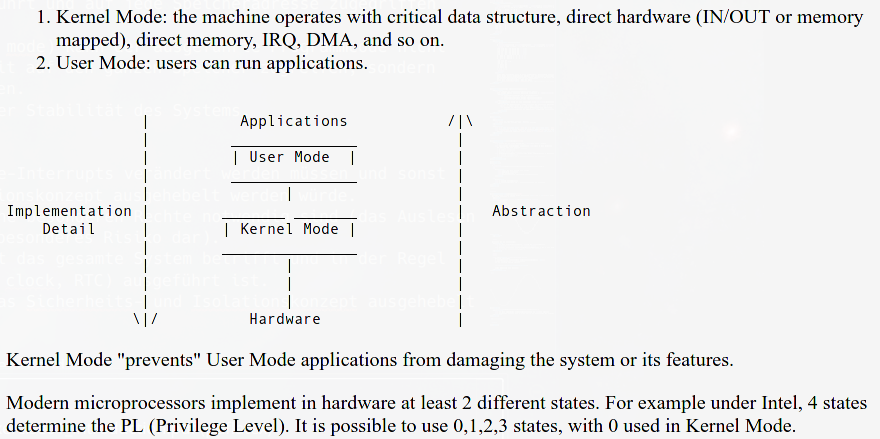
\includegraphics[keepaspectratio, width=0.8\textwidth, height=0.8\textheight-2\baselineskip-2\baselineskip]{img/000_tldp_kernel_user.png} \\
         \caption{The Linux Kernel Documentation Project: Fundamentals~\autocite{tldp_user_kernel}}
        \end{figure}
        \framebreak
        
        \item \textbf{Which of the following instructions should be allowed only in kernel mode, and why?}
			\begin{itemize}
				\item Disabling all interrupts \\
				$\Rightarrow$ \alert{Kernel}, disables interaction HW$\rightarrow$ Kernel
				\item Reading the system clock \\
				$\Rightarrow$ \alert{User}, does not interfere with Kernel or other user programs
				\item Setting the system clock \\
				$\Rightarrow$ \alert{Kernel}, does interfere with Kernel and other user programs that use the system clock 
                \item Changing the memory allocation tables \\
                $\Rightarrow$ \alert{Kernel}, interferes with the memory consistency of Kernel and all other programs
			\end{itemize}
        \framebreak
			
		\item \textbf{Modern operating systems virtualize memory address space, that is, they use logical memory addresses instead of physical (hardware) memory addresses. 
        Describe two advantages of this approach.}
        \begin{itemize}
         \item Can use more memory than physically available (swapping)
         \item Possible to have only necessary parts of program in-memory
         \item Memory isolation: Every program has a separate logical memory space and no access to other addresses
         \item Program memory doesn't need to be physically continuous  (ease allocation)
        \end{itemize}
		\framebreak
        
		\item When a user program reads from a disk file, it becomes blocked until the device driver has finished performing the read operation. Suppose the user program was not blocked when writing to a file, that is, execution of the program would continue while the device driver still performs the write operation.What problem could arise? Can the device driver solve it? \\
		\framebreak
		Problems:
		\begin{itemize}
		 \item What if another thread reads the file before the write?\\
		 Does it get the correct version of the contents? Need a signal for the driver to schedule access
		 \item What if the write failed?
		 \item What if the same program alters the buffer to be written during the write process?
		\end{itemize}
	\end{enumerate}
\end{frame}

\begin{frame}[allowframebreaks]{Exercise 2}
\textbf{What is characteristic for the use of the following types of operating systems?} \\
Operating systems for
\begin{itemize}
 \item personal computers \\
 Responsive, interactive, one user at a time
 \item embedded systems \\
 Few resources, fixed set of programs, reliability, control over device
 \item sensor nodes \\
 Few resources, often only one program to transfer/broadcast data
 \item real-time applications \\
 Hard or soft deadlines for routines, preemptive scheduling, latency of program is fixed within an interval
\end{itemize}
\textbf{What is the difference between timesharing systems and multiprogramming systems?} \\
\begin{itemize}
 \item Timesharing systems: several users run programs on one computing system at the same time.
 \item Multiprogramming systems: users run several programs simultaneously.
\end{itemize}
$\Rightarrow \text{Timesharing} \subset \text{Multiprogramming}$
\end{frame}

\begin{frame}[allowframebreaks]{Exercise 3}
		\begin{enumerate}
			\item \textbf{Complete the table.} C.f. next slide
			\item \textbf{Which quantities are typically specified with binary prefixes?} \\
			Data rates: Transimission speed, Read and Write Speeds. \\
			In general: Digital information.
			\item \textbf{ Why are there no binary prefixes in the lower part of the table?}\\ The bit is the smallest possible chunk of information. There are no "`half"' bits.
			\item \textbf{How large is 1 TB in TiB?} \\
                $\frac {10^{12}}{2^{40}} \sim 0.9094947017729282$
		\end{enumerate}
\framebreak
\begin{minipage}[t][\textheight][t]{\textwidth}
\begin{table}
\begin{center}
	\begin{tabular}[t]{@{}rlclccc@{}}
			\toprule
			& \multicolumn{2}{c}{SI} & \multicolumn{4}{c}{binär} \\ \cmidrule(lr){2-3} \cmidrule(lr){4-7}
			\tiny $b$\,=\,10 & \tiny Name & \tiny Symbol & \tiny Name & \tiny Symbol & \tiny $b$\,=\,2 & \tiny $b$\,=\,1024 \\
			\midrule
			24 & yotta  & Y & yobi & Yi & 80 & 8 \\ % yobi
			21 & zetta  & Z & zebi & Zi & 70 & 7 \\ % zebi
			18 & exa    & E & exbi & Ei & 60 & 6 \\ % exbi
			15 & peta   & P & pebi & Pi & 50 & 5 \\ % pebi
			12 & tera   & T & tebi & Ti & 40 & 4 \\ % tebi
			9 & giga   & G & gibi & Gi & 30 & 3 \\ % gibi
			6 & mega   & M & mebi & Mi & 20 & 2 \\ % mebi 
			3 & kilo   & k & kibi & Ki & 10 & 1 \\ % kibi 
			\hline
			-3 & milli  & m & \\
			-6 & micro  & $\mu$ & \\
			-9 & nano   & n & \\
			 & $\dots$  &  & \\
			\bottomrule
		\end{tabular}
		\caption{Completed table of prefixes from ex. 3}
\end{center}
\end{table}
\end{minipage}
\end{frame}

\begin{frame}[allowframebreaks]{Fetch Decode Execute}
From Patterson \& Hennessy~\autocite{hennessy2011computer}:
	\begin{itemize}
	 \item[A] Fetch current instruction from memory by querying the memory with the program counter/ instruction pointer (RIP/EIP), advance it by the length of an instruction (32/64 bit)
	 \item[B] Decode fetched instruction into micro-code and fetch stored registers from memory if necessary. Compute possible branch targets
	 \item[C] Execute the micro-code instruction. \\ One of: Memory reference - add base and offset, register-register ALU instr. - compute what is spec'ed by op with values from registers, register-immediate ALU instr. - instr. defined second operand like increment or determine whether conditional branch condition is true.
	 \item[D] Memory access: Write result to register or main memory
	\end{itemize}

		\begin{figure}
       \begin{center}
        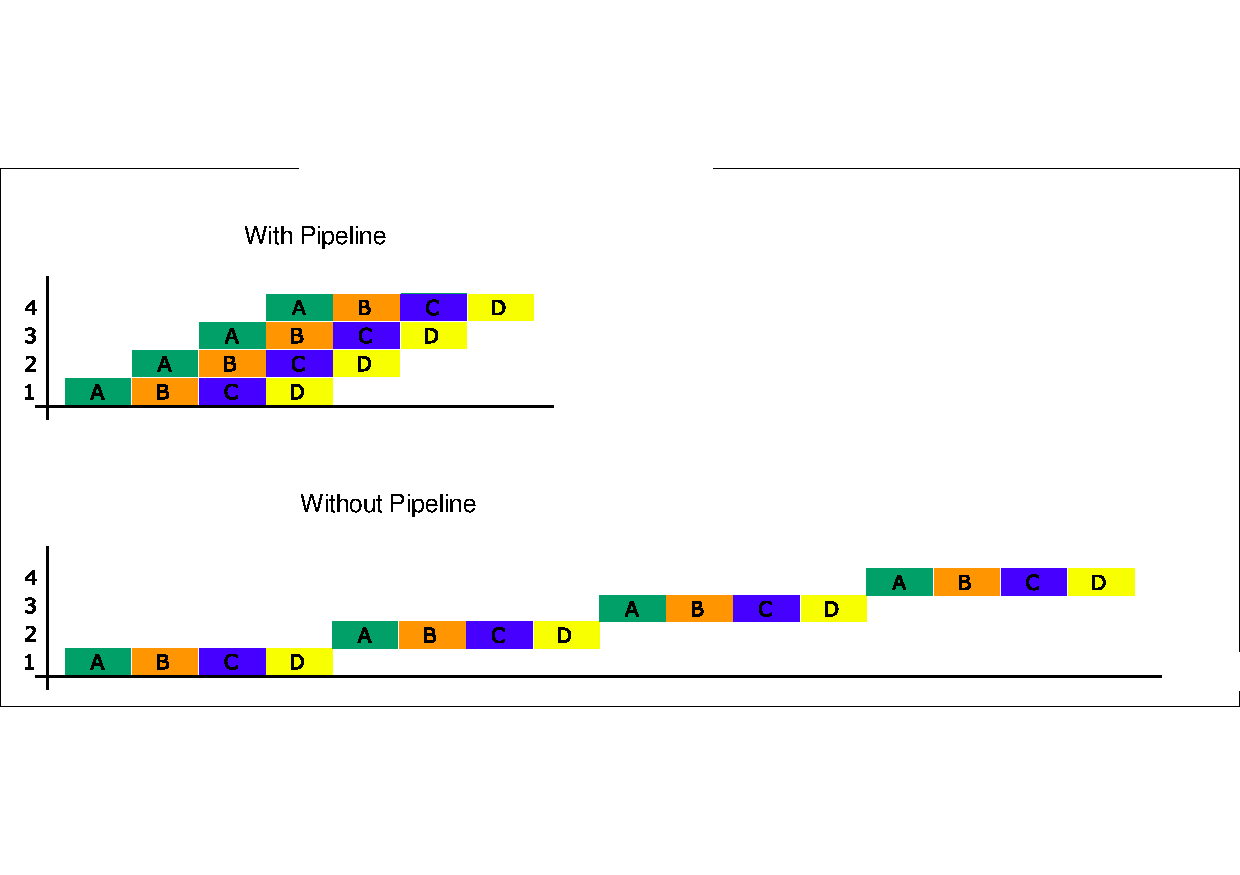
\includegraphics[keepaspectratio, width=\textwidth,height=0.95\textheight-4\baselineskip]{img/Befehlspipeline.pdf} \\
      \end{center}
      \caption{Illustration of instruction pipelining~\autocite{Pipeline}}
      \end{figure} 
      \framebreak
      
      For unpipelined execution engines we have, with $n$ instructions, $k$ steps (here $k = 3$ for fetch decode and execute) and $\tau$ the time one instruction takes:
      \[ n \cdot k \cdot \tau \]
      For pipelined execution engines we get, with $i$ the number of steps before execution (here $i = 2$ for fetch and decode):
      \[ n \cdot \tau - i \]
\end{frame}

\begin{frame}[allowframebreaks]{Exercise 4}
	\begin{enumerate}
		\item A CPU has a three-level fetch-decode-execute pipeline. Each stage of the pipeline takes the same time of \SI{1}{\nano\second} to process.
			\begin{enumerate}
				\item \textbf{How many instructions can the CPU process per second?} \\
				$\frac{1 \text{ instr.}}{\SI{1}{\nano\second}} = \frac{1 \text{ instr.}}{\SI{1}{\second} \cdot 10^{-9}} = 10^9 \cdot 1 \frac{\text{ instr.}}{\si{\second}}$ \\
				1 billion instructions per second.
                
				\item \textbf{How many instructions can the CPU process if the pipelines has five levels?} \\
				Pipelining let's the elements of the FDE cycle operate asynchronous. 
				The same amount, as in pipelines there is only one ALU/element that can execute the operations.  
			\end{enumerate}
        \framebreak
        
        \item A computer system has a cache (access time \SI{2}{\nano\second}), RAM (access time \SI{10}{\nano\second}) and an external storage device (access time \SI{10}{\milli\second}). 
			\begin{enumerate}
				\item \textbf{If the cache hit rate is \SI{95}{\percent} and the main memory hit rate is \SI{99}{\percent}, how long is the average access time?} \\
 				$0.95 \cdot \SI{2}{\nano\second} + 0.05 \cdot (0.99 \cdot \SI{10}{\nano\second} + 0.01 \cdot \SI{10}{\milli\second}) =  \SI{5002.39}{\nano\second} \sim \SI{5}{\micro\second}$
				
				\item \textbf{Which of the three access times dominates the average access time?} \\
				External memory as it is slower by orders of magnitude.
				
				\item \textbf{Another external memory device is connected. The measured average access time is now \SI{2002.395}{\nano\second}. 
                    What is the access time of the new external storage device?}  \\
                    $ \SI{2002.395}{\nano\second} = 0.95 \cdot \SI{2}{\nano\second} + 0.05 \cdot (0.99 \cdot \SI{10}{\nano\second} + 0.01 \cdot x \si{\milli\second}) $\\
                    Solving for $x$ yields $x = \SI{3996000}{\nano\second} \sim \SI{4}{\milli\second}$
			\end{enumerate}
	\end{enumerate}

\end{frame}

\begin{frame}[allowframebreaks]{Exercise 5}
    \begin{enumerate}
		\item \textbf{Write a \mintinline{c}{C} program that outputs ``\texttt{Hello world!}''.} \\ \vspace{1cm}
			\inputminted{c}{code/hello_world.c}
			\framebreak
		\item \textbf{Compile your program using the flags \mintinline{bash}{-std=c11 -g -Wall -Wpedantic}.
			What does each of these flags mean?}
			\begin{itemize}
			 \item -std=c11 the 2011 ISO C standard
			 \item -g debugging information
			 \item -Wall turn on lots of error checking
			 \item -Wpedantic strict ISO C conformity
			\end{itemize}
			\framebreak
		\item \textbf{Which additional files are generated when you use the \mintinline{bash}{-save-temps} flag and what do they contain?}
		\begin{itemize}
		 \item .i generated by the pre-processor, source with expanded pre-processor directives
		 \item .s generated assembly code by the compiler
		 \item .o generated machine code by the assembler
		 \item .out generated executable by the linker
		\end{itemize}
	\end{enumerate}
	

\end{frame}

\begin{frame}[allowframebreaks]{Exercise 6}
    Write a \mintinline{c}{C} program that outputs the sine function $\sin(x)$ for $x \in [0,2\pi]$ on the console.
    \framebreak
    \begin{mdframed}[linecolor=black, topline=false, bottomline=false,
  leftline=false, rightline=false, backgroundcolor=lg]
    \inputminted[fontsize=\tiny, linenos, frame=lines]{c}{code/sin.c}
\end{mdframed}
    \framebreak
    \begin{mdframed}[linecolor=black, topline=false, bottomline=false,
  leftline=false, rightline=false, backgroundcolor=lg]
    \inputminted[fontsize=\tiny, linenos, frame=lines]{c}{code/sin-alt.c}
\end{mdframed}
\end{frame}
    
\section{Exercise sheet 2}
\frame{\sectionpage}
\begin{frame}[allowframebreaks]{}
 \begin{figure}
         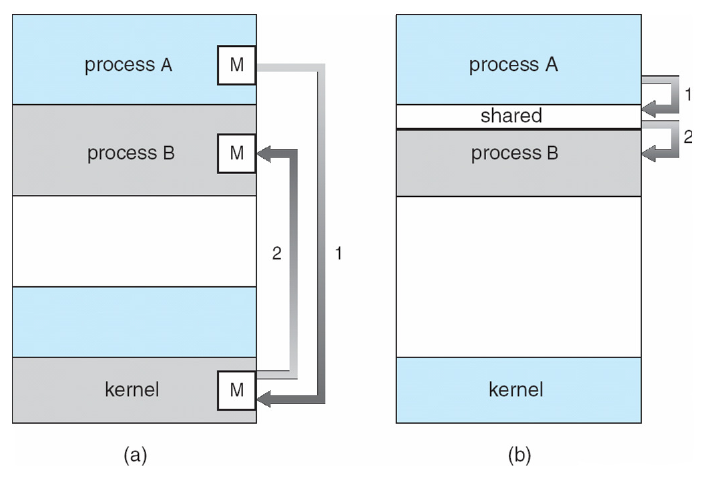
\includegraphics[keepaspectratio, width=0.8\textwidth, height=0.8\textheight-2\baselineskip-2\baselineskip]{img/012_mem_map.png} \\
         \caption{Visualization of how the kernel logically maps the main memory~\autocite{silberschatz}}
        \end{figure}
        \framebreak
        \begin{figure}
         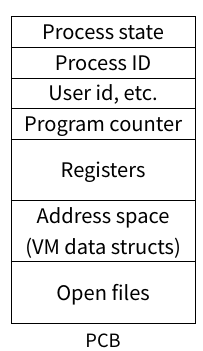
\includegraphics[keepaspectratio, width=0.8\textwidth, height=0.8\textheight-2\baselineskip-2\baselineskip]{img/010_pcb.png} \\
         \caption{Elements contained in a process control block~\autocite{tanenbaum}}
        \end{figure}
        \framebreak
        \begin{figure}
         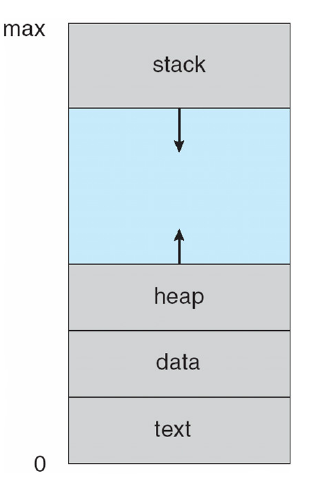
\includegraphics[keepaspectratio, width=0.8\textwidth, height=0.8\textheight-2\baselineskip-2\baselineskip]{img/010_process_memory.png} \\
         \caption{Elements contained in a process control block~\autocite{silberschatz}}
        \end{figure}
        \framebreak
        \begin{figure}
         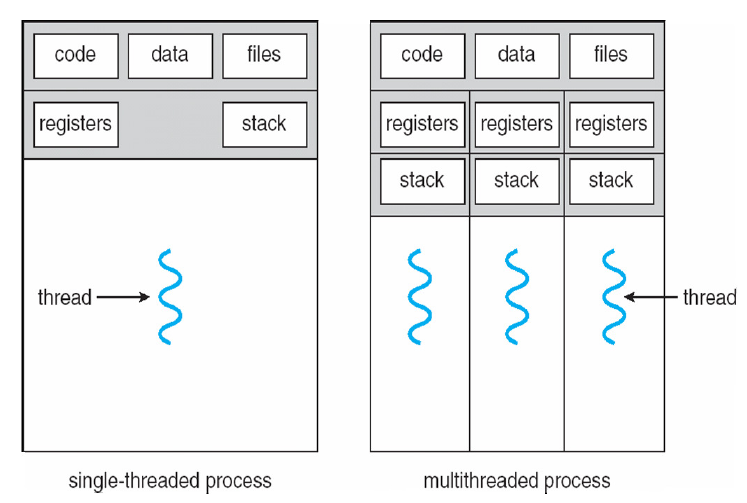
\includegraphics[keepaspectratio, width=0.8\textwidth, height=0.8\textheight-2\baselineskip-2\baselineskip]{img/010_proc_threads.png} \\
         \caption{Elements contained in a process control block~\autocite{silberschatz}}
        \end{figure}
\end{frame}


\section{C}
\frame{\sectionpage}
\begin{frame}{Memory is uninitialized!}
\begin{itemize}
 \item \href{https://wiki.sei.cmu.edu/confluence/display/c/EXP33-C.+Do+not+read+uninitialized+memory}{https://wiki.sei.cmu.edu/confluence/display/c/EXP33-C.+Do+not+read+uninitialized+memory}
 \item C Arrays
\end{itemize}

 
\end{frame}

\section{References}
    \begin{frame}[allowframebreaks]
      \frametitle{References}
      \begin{tiny}
      \nocite{*}
      \printbibliography
      \end{tiny}
    \end{frame}


\end{document}
 
